\chapter{Marco Metodológico}
\section{Proceso de Obtención de Datos}
El proceso de obtención de datos para el entrenamiento de los algoritmos se realizó por medio de entrevistas a distintos individuos. La población objetivo para estas entrevistas se delimitó a estudiantes y colaboradores de la Universidad del Valle de Guatemala. El proceso de extracción de información se realizó mediante pruebas dentro de estas entrevistas, a las cuales los individuos de estudio se ofrecían voluntariamente para tomarlas mediante una solicitud con un formulario electrónico en línea. Estas pruebas fueron realizadas en un ambiente controlado dentro de las instalaciones de las Clínicas de Psicología de la Universidad del valle de Guatemala, durante los meses de marzo y abril del año 2018. 

Estas entrevistas se realizaron a cincuenta y seis (56) sujetos pertenecientes al grupo de estudio objetivo. Un estudio con un número de participantes mayor a veintidós puede aportar mejores resultados (Davatzikos et al., 2005). Cada participante proporcionó algunos datos personales para determinar datos  sobre la población en la cual se realizó el experimento. Estos datos incluyen género, edad, lateralidad, escolaridad, grupo étnico, estado civil, sector de población universitaria a la que pertenecen, empleo y acompañamiento psicológico. De igual manera, se realizaron pruebas psicometrícas a los individuos de estudio durante el proceso de entrevista, acompañados por estudiantes de la facultad de Psicología. Además que estos datos permiten determinar posibles variables relacionadas con el engaño, estos también pueden ser útiles para las personas que deseen utilizar el conjunto de datos para otros estudios o para continuar el presente trabajo.

Durante las entrevistas realizadas, se pidió a los participantes responder a una serie de preguntas seleccionadas que un moderador les realizaría. Estas preguntas se realizaron durante dos rondas. En la primera ronda, se solicitó al sujeto que respondiera a las preguntas diciendo la verdad. En la segunda ronda, se realizaron las mismas preguntas, pero se solicitó al sujeto que respondiera con falacias. Durante estas rondas de preguntas, la extracción de la información se realizó por medio de distintos instrumentos de medición relacionados a los módulos del proyecto. Las entrevistas fueron grabadas con vídeo y audio, además de utilizar los instrumentos de medición de ondas electroencefalográficas.

La obtención de datos de la actividad electroencefalográfica de los sujetos se realzó mediante el uso de un casco \textit{Emotiv EPOC} y su conexión a un ordenador con el panel de control \textit{Emotiv Xavier}. El uso del dispositivo para la extracción de la información se hizo empleando el proyecto \textit{EMOTRIX}. El proyecto Emotrix es una plataforma que permitirá el estudio, identificación y manipulación de emociones humanas. La plataforma se podrá utilizar para fines educativos, médicos o recreacionales, entre otros. A la fecha, existen distintos dispositivos que permiten imitar inteligencia emocional, los cuales tienen precios elevados. Es por esto por lo que la plataforma tiene un enfoque de código libre para permitir el desarrollo de forma abierta y evitar cualquier tipo de restricciones a los usuarios. El ámbito al que pertenece el proyecto es a la interacción humano – computador (HCI). Este proyecto ha sido desarrollado desde 2016 por estudiantes de la Universidad del Valle de Guatemala.

\section{Análisis Exploratorio de los Datos}

Se obtuvieron una serie de variables de distintos tipos procedentes de las pruebas realizadas en las entrevistas. Se obtuvieron quince (15) variables procedentes de Emotiv EPOC, referentes a los canales de lectura del mismo. Se obtuvieron doce (12) variables descriptivas de los individuos entrevistados y de sus pruebas psicométricas asociadas. Estas últimas son género, edad, lateralidad, escolaridad, grupo étnico, estado civil, prueba l1 ,prueba l2, sector de la población de la universidad a la que pertenecen, empleo, acompañamiento psicológico y tipo de acompañamiento psicológico. Para un total de veintisiete variables. De las variables electroencefalográficas, se tomó únicamente las que procedían de los transmisores ubicados en los lóbulos frontales. Esto se debe a que se sugiere que las emociones relacionadas con el engaño se encuentran en esta parte del cerebro humano (Belmonte C., 2007). Por lo que se trabajaron ocho (8) variables de este tipo, referente a los canales AF3, AF4, F3, F4, F7, F8, FC5 y FC6. 

\begin{figure}
    \centering
    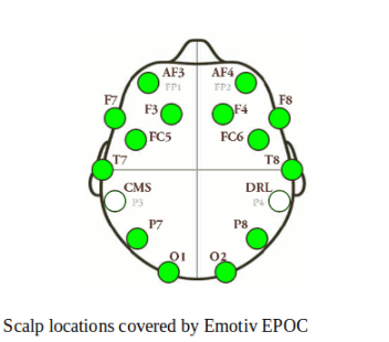
\includegraphics[scale=1]{figuras/Imagen3.png}
    \caption{Las posiciones de los electrodos EPOC en la cabeza se aproximan al sistema internacional 10-20.}
    \label{fig:my_label}
\end{figure}

\begin{table}
    \centering
    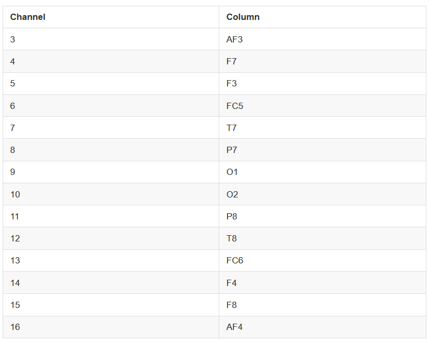
\includegraphics[scale=1]{figuras/Imagen4.png}
    \caption{Electrodos EPOC con su canal de salida respectivo.}
    \label{tab:my_label}
\end{table}

A partir de estas variables obtenidas, se realizaron análisis de regresión logística y de árboles de decisión para poder identificar a las variables más significativas para alimentar los modelos de predicción. Mediante estas técnicas, se buscaría reducir el número de características que el modelo llegaría a procesar. Del mismo modo, se realiza un análisis de \textit{wavelets} que permite identificar la frecuencia con mayor presencia y su punto de ocurrencia a lo largo del tiempo. Estas frecuencias indican predominancia de las ondas electroencefalográficas a lo largo de las mediciones. Estos análisis se realizaron empleando el lenguaje de programación R y el software \textit{RStudio}.

\begin{figure}
    \centering
    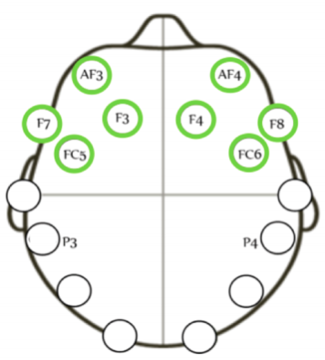
\includegraphics[scale=0.92]{figuras/Imagen2.png}
    \caption{Electrodos EPOC a considerar para la selección de variables.}
    \label{fig:my_label}
\end{figure}

\section{Construcción del Conjunto de Datos de Entrenamiento}
El conjunto de datos de entrenamiento se generó a partir de las variables obtenidas del análisis exploratorio de los datos. Este conjunto de datos se construye por medio de la unión de las variables electroencefalográficas y las variables descriptivas del sujeto. El conjunto de datos sin análisis exploratorio logró reducirse en trece (13) variables. En cuanto al numero de tuplas de observaciones obtenidas, el conjunto de datos se redujo de aproximadamente un millón quinientos mil (1,500,000) a novecientas mil (900,000) aproximadamente. De tal forma que los datos fueron almacenados para luego poder ser unidos con los respectivos resultados de las pruebas descriptivas. 

Para la generación de los conjuntos de datos procedentes de los resultados obtenidos, se utilizó el lenguaje de programación \textit{Python}. Se utilizó la librería \textit{pandas} para la extracción de los datos procedentes de archivos de texto separados por comas (CSV). Se empleó la librería de expresiones regulares \textit{re} nativa de Python para poder procesar la información procedente de los archivos de Emotiv EPOC. Además de contener las variables estudiadas, se añadió la variable dependiente de mentira al conjunto de datos destinado a entrenamiento. Esta variable describe a los datos procedentes de cuando una persona estaba mintiendo o no, para poder clasificar los datos. Esta variable representa a las observaciones de verdad con un cero (0) y a las de mentira con un uno (1). 

El conjunto de datos de entrenamiento se dividió dos grupos: la parte destinada a entrenar a los algoritmos predictivos, y otra parte para realizar pruebas de precisión. El grupo de entrenamiento está compuesto por el setenta (70) por ciento de los datos totales. El grupo de prueba está formado por el restante treinta (30) por ciento. En los algoritmos de aprendizaje de máquina, se aplicó el método de $\epsilon$ pliegos para implementar validación cruzada. Este método se empleó con los tamaños de entrenamiento y prueba descritos con anterioridad.     

\section{Desarrollo del Modelo de Clasificación}
Los modelos de aprendizaje de máquina se implementaron utilizando el lenguaje de programación \textit{Python 3.6.0}. Se utilizaron las librerías \textit{pandas, numpy, Scikit-Learn y TensorFlow} para realizar diversas implementaciones de los algoritmos de Máquinas de Vectores de Soporte. Estos algoritmos toman como entrada el conjunto de datos generado en la construcción del conjunto de datos de entrenamiento. La lectura de los archivos de entrenamiento se realizó por medio de la librería \textit{pandas}. Las gráficas que permitieron realizar análisis de precisión y rendimiento se realizaron empleando la librería \textit{matplotlib}. Se desarrolló el modelo empleando un ambiente virtual de Python, el cual se trabajó un sistema operativo \textit{Xubuntu 18.04}, basado en \textit{Debian}.

Se implementó la librería \textit{TensorFlow} de \textit{Google} para realizar los algoritmos de aprendizaje de máquina. Esta librería resuelve el problema de convergencia utilizando segmentos del conjunto de datos para realizar los cálculos matemáticos. La iteración de estos cálculos a partir de distintos segmentos llega a aproximar lo que sería el procesamiento del grupo completo del conjunto de datos. 

La comparación de la precisión de predicción de los algoritmos de máquina empleados permite determinar el mejor algoritmo para esta tarea. La salida de los algoritmos desarrollados es entonces la precisión de la detección del engaño y la detección misma del engaño a partir de un conjunto de entrada. La salida de un conjunto de datos de una predicción en tiempo real estaría formada por un valor único, que representa si la persona mintió o no a lo largo de la prueba, y un valor de certeza. Este último estaría dado por la cantidad de valores repetidos de predicción por cada una de las observaciones del sujeto.  

\section{Desarrollo del la Interfaz de Respuesta}
La interfaz de usuario se realizará utilizando el framework \textit{Vue.js} y en lenguaje \textit{Javascript}, para realizar la parte visual y de muestra de datos al usuario que emplee el sistema. El servidor que realizará las llamadas a los módulos desarrollados, incluyendo este, se realizará en el framework \textit{Flask}, el cual emplea el lenguaje de programación \textit{Python}. El objetivo de estas tecnologías es brindar una conexión sencilla entre la obtención de datos, su procesamiento en módulos, y su posterior presentación al usuario.

El diseño de esta interfaz se enfoca en la simplicidad y facilidad de uso de la misma. Con el objetivo de ser utilizada por los estudiantes de la facultad de Psicología de la Universidad del Valle pertenecientes al proyecto. De esta forma, se busca que una persona ajena al ambiente de desarrollo tecnológico utilice el sistema para predecir el engaño frente a un sujeto de prueba. Estos objetivos se verificarán al momento de dar uso al sistema por parte de estos estudiantes durante un período de prueba del sistema, luego de su desarrollo.


\chapter{Resultados}
\section{Conjunto de Datos de Entrenamiento}
Al finalizar la recolección de datos de entrenamiento para la creación de los modelos se obtuvo los siguientes resultados de las características exploradas de los cincuenta y seis (56) sujetos de la población objetivo:
\begin{figure}
    \centering
    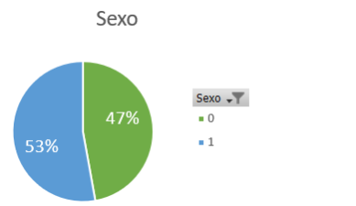
\includegraphics[scale=1]{figuras/Imagen11.png}
    \caption{Género de los sujetos de la población de estudio. Cero (0) representa Femenino, uno (1) masculino.}
    \label{fig:my_label}
\end{figure}
\begin{figure}
    \centering
    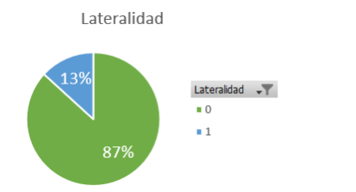
\includegraphics[scale=1]{figuras/Imagen12.png}
    \caption{Lateralidad de los sujetos de la población de estudio. Cero (0) representa diestro, uno (1) representa zurdo.}
    \label{fig:my_label}
\end{figure}
\begin{figure}
    \centering
    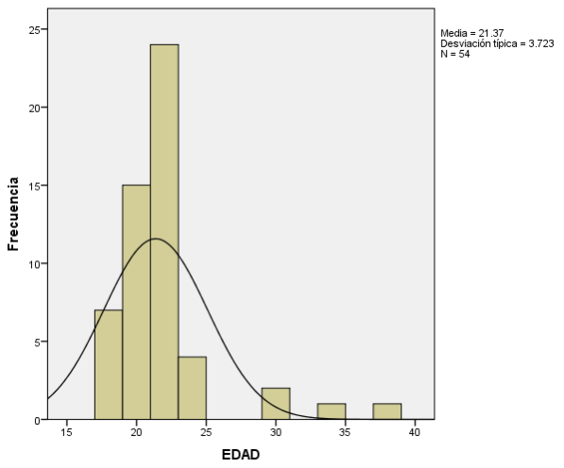
\includegraphics[scale=0.85]{figuras/Imagen14.png}
    \caption{Distribución de la edad de los sujetos de la población de estudio.}
    \label{fig:my_label}
\end{figure}
\begin{figure}
    \centering
    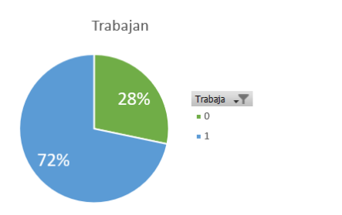
\includegraphics[scale=1]{figuras/Imagen15.png}
    \caption{Situación laboral de los sujetos de la población de estudio.}
    \label{fig:my_label}
\end{figure}
\begin{figure}
    \centering
    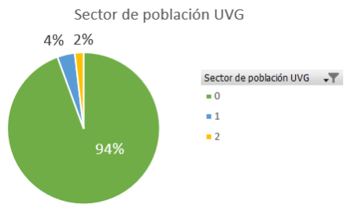
\includegraphics[scale=1]{figuras/Imagen16.png}
    \caption{Sector de la población universitaria a la que pertenecen los sujetos de estudio. Cero (0) representa estudiante, uno (1) personal administrativo, dos (2) personal docente.}
    \label{fig:my_label}
\end{figure}
\begin{figure}
    \centering
    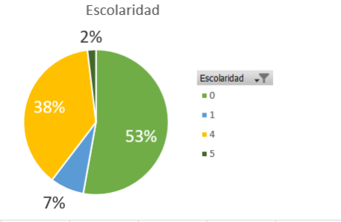
\includegraphics[scale=1]{figuras/Imagen17.png}
    \caption{Escolaridad de los sujetos de la población de estudio. Cero (0) representa diversificado, uno (1) Diplomado, dos (2) pregrado, tres (3) maestría. }
    \label{fig:my_label}
\end{figure}
\begin{figure}
    \centering
    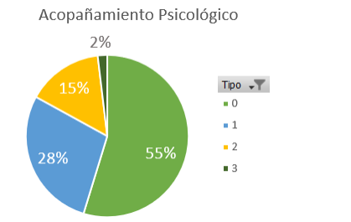
\includegraphics[scale=1]{figuras/Imagen18.png}
    \caption{Acompañamiento psicológico de los sujetos de la población de estudio. Cero (0) representa ninguno, uno (1) terapia, dos (2) consejería, tres (3) evaluación}
    \label{fig:my_label}
\end{figure}
\begin{figure}
    \centering
    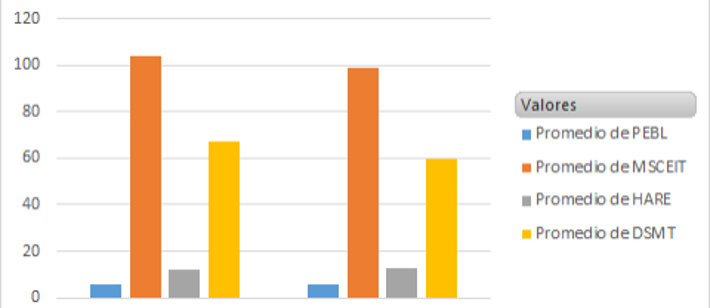
\includegraphics[scale=0.70]{figuras/Imagen19.png}
    \caption{Promedio de resultados de las pruebas psicométricas realizadas por los sujetos de la población de estudio.}
    \label{fig:my_label}
\end{figure}
A continuación, se presentan muestras de los resultados del análisis electroencefalográfico de los sujetos pertenecientes a la población de estudio, obtenidos por Emotiv EPOC:  
\begin{figure}
    \centering
    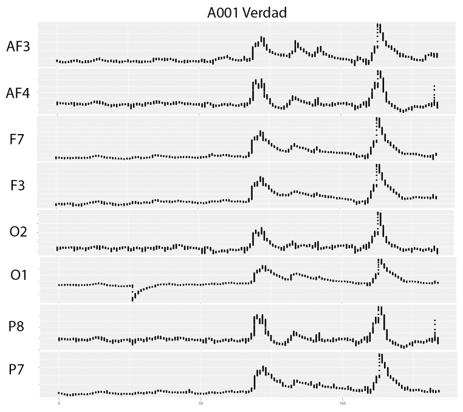
\includegraphics[scale=0.75]{figuras/Imagen5.png}
    \caption{Datos provenientes de los canales de Emotiv EPOC para verdad, de uno de los sujetos de prueba (A001).}
    \label{fig:my_label}
\end{figure}
\begin{figure}
    \centering
    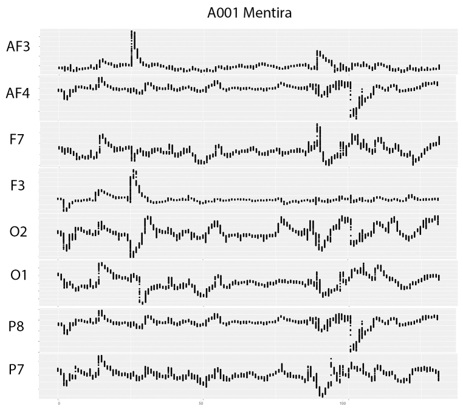
\includegraphics[scale=0.75]{figuras/Imagen6.png}
    \caption{Datos provenientes de los canales de Emotiv EPOC para mentira, de uno de los sujetos de prueba (A001).}
    \label{fig:my_label}
\end{figure}
\begin{figure}
    \centering
    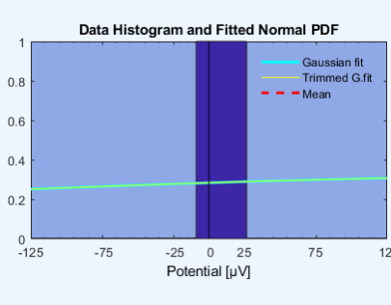
\includegraphics[scale=1]{figuras/Imagen7.png}
    \caption{Histograma de los datos de verdad del canal AF3 de uno de los sujetos de prueba (A001).}
    \label{fig:my_label}
\end{figure}
\begin{figure}
    \centering
    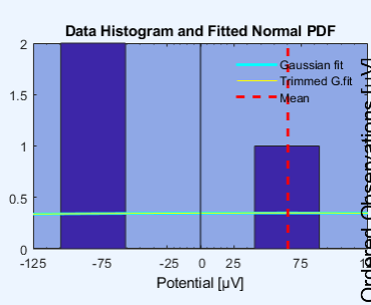
\includegraphics[scale=1]{figuras/Imagen8.png}
    \caption{Histograma de los datos de mentira del canal AF3 de uno de los sujetos de prueba (A001).}
    \label{fig:my_label}
\end{figure}
\begin{figure}
    \centering
    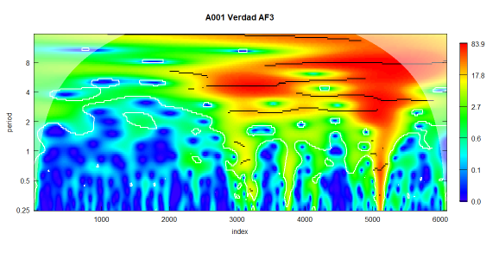
\includegraphics[scale=1]{figuras/Imagen9.png}
    \caption{Gráfico de Wavelets de los datos de verdad de uno de los sujetos de prueba (A001).}
    \label{fig:my_label}
\end{figure}
\begin{figure}
    \centering
    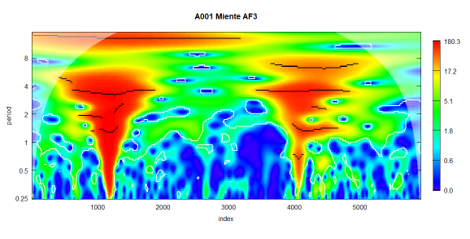
\includegraphics[scale=1]{figuras/Imagen10.png}
    \caption{Gráfico de Wavelets de los datos de mentira de uno de los sujetos de prueba (A001).}
    \label{fig:my_label}
\end{figure}
\section{Análisis Exploratorio de Variables}
A estas variables se les realizó un análisis de regresión logística y de árboles de decisión para obtener las más significativas para el estudio. Los resultados de estos análisis se muestran a continuación:
\begin{figure}
    \centering
    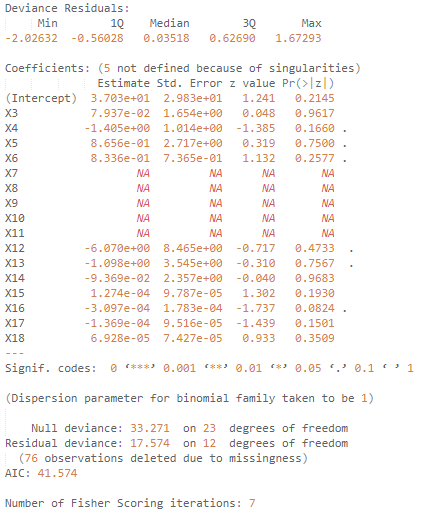
\includegraphics[scale=1.05]{figuras/Capture4.PNG}
    \caption{Resultados del análisis de regresión logística.}
    \label{fig:my_label}
\end{figure}
\begin{figure}
    \centering
    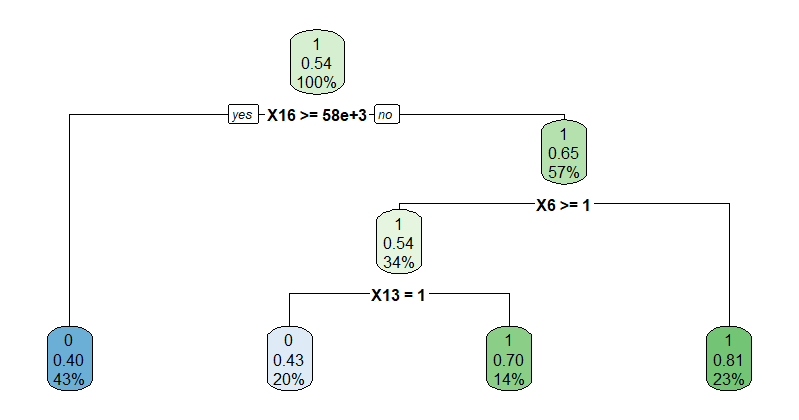
\includegraphics[scale=0.65]{figuras/Rplot1.png}
    \caption{Resultados del análisis de árbol de decisión.}
    \label{fig:my_label}
\end{figure}
\begin{figure}
    \centering
    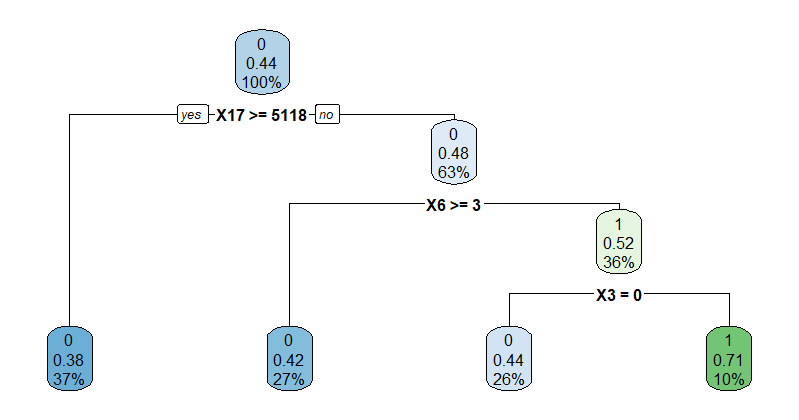
\includegraphics[scale=0.65]{figuras/Rplot2.png}
    \caption{Resultados del análisis de árbol de decisión.}
    \label{fig:my_label}
\end{figure}
A partir de estos resultados, se obtuvieron las variables más significativas para poder entrenar los algoritmos de aprendizaje de máquina. Estas son un total de catorce (14) variables, ocho (8) de electroencefalograma y seis (6) de variables descriptivas. Estas variables descriptivas son: edad, lateralidad, escolaridad, empleo y acompañamiento psicológico. La variable más significativa fue la relacionada a el canal F3 de Emotiv EPOC.
\section{Precisión de las Máquinas de Vectores de Soporte}
Los resultados de la precisión de las distintas Máquinas de Vectores de Soporte, alimentadas por las variables seleccionadas, se presentan a continuación: 
\begin{figure}
    \centering
    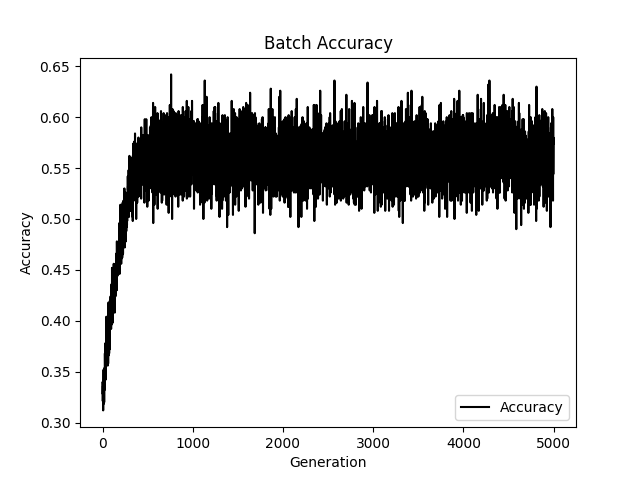
\includegraphics[scale=0.75]{figuras/Figure_1.png}
    \caption{Precisión de la Máquina de Vectores de Soporte con kernel RBF.}
    \label{fig:my_label}
\end{figure}
\begin{figure}
    \centering
    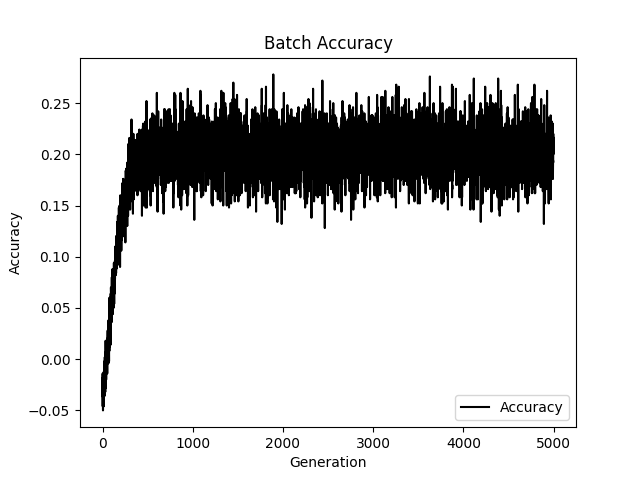
\includegraphics[scale=0.75]{figuras/Figure_2.png}
    \caption{Precisión de la Máquina de Vectores de Soporte con kernel Lineal.}
    \label{fig:my_label}
\end{figure}
\begin{figure}
    \centering
    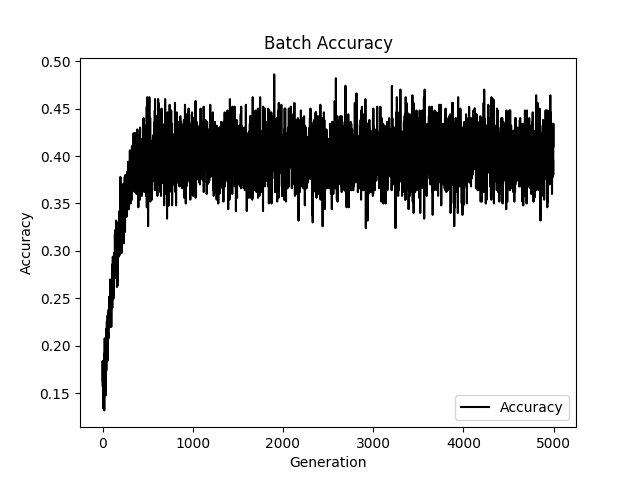
\includegraphics[scale=0.75]{figuras/Figure_3.png}
    \caption{Precisión de la Máquina de Vectores de Soporte con kernel Polinomial.}
    \label{fig:my_label}
\end{figure}
La siguiente figura muestra la precisión de la Máquina de Vectores de Soporte con distintos valores de $C$ y $\gamma$. Los valores que brindaron la mejor precisión en la predicción del engaño fueron los que se emplearon como valores finales.
\begin{figure}
    \centering
    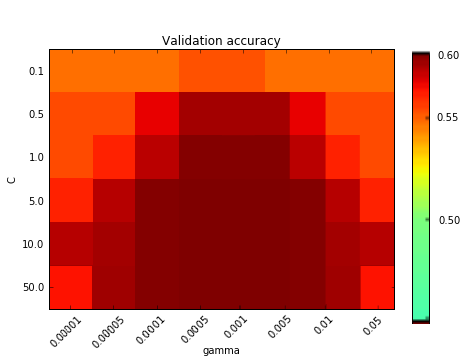
\includegraphics[scale=1]{figuras/58e171451b12ce00012bd71d.png}
    \caption{Precisión de la Máquina de Vectores de Soporte con kernel RBF con distintos valores de $C$ y $\gamma$.}
    \label{fig:my_label}
\end{figure}
\section{Interfaz de Sistema de Detección del Engaño}
El diseño de la interfaz del usuario para el sistema de detección del engaño se desarrolló en conjunto con los distintos integrantes de los módulos del proyecto. El esquema de lo que sería la interfaz principal se muestra a continuación.
\begin{figure}
    \centering
    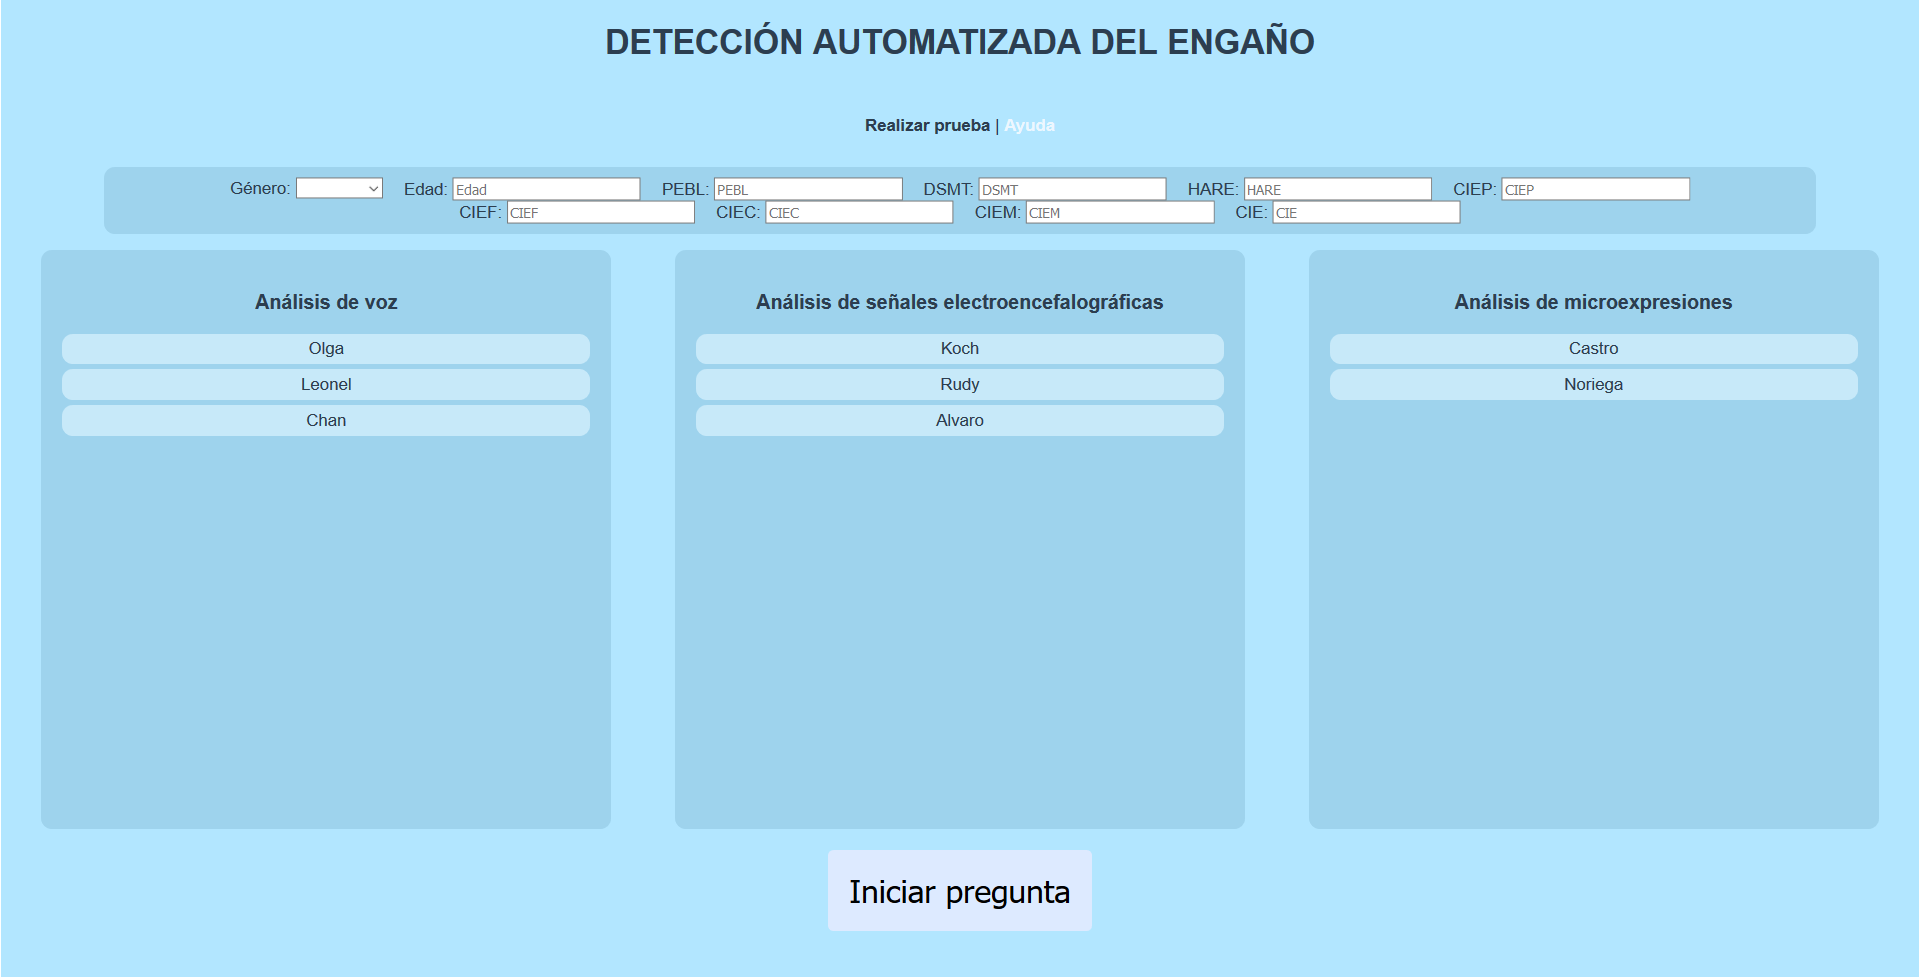
\includegraphics[scale=0.42]{figuras/Imagen20.PNG}
    \caption{Interfaz de uso del sistema de detección del engaño.}
    \label{fig:my_label}
\end{figure}
El objetivo de este diseño es proporcionar a una persona con limitados conocimientos en el sistema una interfaz sencilla, amigable y suficientemente explícita para poder comparar los distintos valores de precisión cuando se realiza una prueba en un sujeto. 

\chapter{Análisis de Resultados}
El análisis exploratorio dejó como resultados variables como la edad, la lateralidad, la escolaridad, el empleo y el acompañamiento psicólogico como significativas para la detección del engaño. Además, el canal F3, que hace referencia a el lóbulo frontal izquierdo del cerebro, parece tener un valor mayor de significancia respecto a los demás canales, de acuerdo a los resultados obtenidos por la regresión logística. Sin embargo, este valor no es demasiado distinto al de los demás canales estudiados, como el canal AF3 y AF4. El valor Pr asociado a estas variables es de 0.08 para el canal F3, 0.19 para el canal AF3 y 0.15 para el canal AF4. Estos valores son los más cercanos al valor de significancia asociado, 0.05. Por lo que a pesar que el valor de F3 fue el más cercano a este, este valor no es muy distinto al de estos otros canales.

Para apoyar estos resultados, se puede apreciar en los árboles de decisión seleccionados que las variables electroencefalográficas como F3 y AF4 se encuentran en la parte más alta de los mismos. Lo cual indica un mayor peso con respecto a otras variables. Se puede obtener de ellas, además, de variables como \textit{escolaridad} sobresalen de otras variables descriptivas. A partir de estos resultados, se puede ver que las variables descriptivas de mayor significancia fueron: edad, escolaridad, empleo y acompañamiento psicológico. 

La causa de estas variables descriptivas como posibles valores referentes del engaño puede deberse a que, por ejemplo, una persona sin empleo puede desarrollar técnicas para presentar mejores atribuciones al momento de presentarse una oportunidad laboral. Un niño puede no tener la suficiente experiencia de vida como para evadir ser detectado al momento de decir una mentira. Sin embargo, estas solo son especulaciones y es necesario pruebas más exhaustivas para poder llegar a relacionar por completo estas características con el engaño en su totalidad.

Respecto a las variables electroencefalográficas, el canal F3 fue el más representativo. Sin embargo, ésta no fue mucho mayor que los canales AF3 y AF4. Este es un resultado esperado debido a la posición en la que tomaron la información estos canales. El lóbulo frontal del cerebro sugiere ser el foco en donde ocurren emociones relacionadas con el engaño. Además, la varianza en los datos obtenidos cuando un sujeto mentía se pudo apreciar de gran manera durante el análisis de estos datos. Esto sugiere una variación de señales electroencefalográficas mayor cuando una persona intenta engañar. El análisis de wavelets permite identificar los tiempos en donde esta actividad tuvo una mayor presencia. Esto es de importancia al momento de seleccionar los datos más significativos para el estudio.

Por otro lado, se empleó en una primera instancia \textit{Scikit-learn} para la implementación de los algoritmos. Sin embargo, debido a las dimensiones del conjunto de datos, el tiempo de convergencia del algoritmo fue demasiado grande para los fines del proyecto. Esto se debe a que el tiempo de convergencia escala entre $O$($n_caracteristicas x n_muestras^2$) y $O$($n_caracteristicas x n_muestras^3$). Es por esta razón que la implementación de esta librería se recomienda para muestras menores a diez mil (10,00) observaciones. De esta forma, el uso de la librería \textit{TensorFlow} permitió un tiempo de convergencia menor para estos algoritmos utilizando el conjunto de datos seleccionado. 

Los resultados de la precisión de los algoritmos de máquina de vectores de soporte indican una clara mayor precisión por parte del algoritmo con kernel gaussiano RBF. Debido a la naturaleza de los datos, se esperaba que el kernel lineal tuviese baja precisión. El kernel polinomial no arrojó una precisión suficientemente elevada como para considerarse \textit{"bueno"}. Esto puede deberse a la naturaleza de los distintos tipo de datos utilizados. A pesar de poder haber sido modelado, la complejidad de estos al utilizarse en conjunto pudo haber causado un \textit{overfitting} del modelo con estos datos, reduciendo la precisión de predicción al momento de utilizar datos nuevos.

La precisión del kernel gaussiano RBF se vio mejorada con valores de $\gamma$ cercanos a $2^{-9}$ y de $C$ cercanos a $2^{3}$. Sin embargo, esta precisión no se vio ampliamente mejorada con respecto a otros valores empleados. Dejando cincuenta y ocho (58) por ciento de precisión como mejor valor predictivo de los datos. A pesar de ser un valor alto para este tipo de pruebas, se vio un mucho mejor rendimiento con el algoritmo \textit{K Vecinos Cercanos} empleando en otro módulo de análisis electroencefalográfico del proyecto. Por lo cual, a pesar de que Máquina de Vectores de Soporte logra un valor de predicción aceptable, se recomienda emplear K Vecinos Cercanos para el análisis electroencefalográfico en la detección del engaño.

El desarrollo de interfaz para el uso del los algoritmos de predicción tuvo por objetivo el uso de simplicidad y facilidad de uso. Se pensó en estudiantes de Psicología que acompañan el proyecto como la población objetivo de su uso. Sin embargo, para generalización del sistema, debe de realizarse un diseño más exhaustivo que permita a cualquier persona, ya sea afín a una ciencia humana o sin conocimiento alguno del uso de la tecnología, poder emplear correctamente el sistema. 

El desarrollo de esta interfaz se realizó por medio de \text{Vue.js}, un framework de \textit{Javascript}. Esta tecnología fue elegida por la versatilidad y simplicidad que tiene para poder conectarse con otras tecnologías. El servidor principal, desarrollado en el framework \textit{Flask} y basado en el lenguaje de programación Python, se enfoca también en la utilización de un servidor simple pero con gran poder computacional. Estas tecnologías fueron seleccionadas entonces por su facilidad de uso y compatibilidad con otras tecnologías. 

El enfoque de la interfaz de usuario, el cual fue simplista y fácil de usar, fue corroborado por los estudiantes de Psicología del proyecto al momento de realizar las pruebas del sistema con usuarios reales. A pesar de desarrollarse de esta manera, se hizo énfasis por parte de los mismos de no ser completamente intuitiva en su primer uso. La carencia de un flujo explícito de su uso dentro de la interfaz puede ser motivo por el cual pueda generarse una curva de aprendizaje considerable. 

Esta carencia de uso intuitivo puede afrontarse colocando un flujo de usuario más explícito. Por ejemplo, colocando botones distintos separados de izquierda a derecha para ejemplificar de manera de flujo lo que el usuario debe realizar. De igual manera, colocar colores opacos en los botones inactivos puede brindar al usuario un mejor enfoque de lo que debe de realizar al hacer la pruebas con usuarios reales. El uso de colores significativos puede apoyar estas decisiones. Estas mejoras pueden hacer de la interfaz de usuario del sistema una herramienta con mayor facilidad de uso. 

%\section{Dinámica de cuerpos rígidos}
%\section{Restricciones}
%\subsection{Mecanismos de lazo cerrado}
%\subsubsection{Mecanismo de cuatro barras}
%\chapter{Control del sistema mecánico}
%\section{La ecuación del manipulador}